\problemset{Теория вероятностей и математическая статистика}
\problemset{Индивидуальное домашнее задание №4}

% Команда ниже задает "название" или слово, которое будет
% отображаться вместо proof или "доказательство"
% поскольку у нас в ИДЗ задачи - то нужно слово "Решение"
\renewcommand*{\proofname}{Решение}
Матрица вероятностей перехода однородной цепи Маркова имеет вид
\[
P = \frac{1}{10}\begin{pmatrix}
    0 & 0 & 0 & 0 & 4 & 6 \\
    0 & 0 & 0 & 0 & 3 & 7 \\
    0 & 3 & 1 & 0 & 6 & 0 \\
    0 & 0 & 0 & 3 & 7 & 0 \\
    7 & 3 & 0 & 0 & 0 & 0 \\
    7 & 3 & 0 & 0 & 0 & 0 \\
\end{pmatrix}
\]

%%%%%%%%%%%%%% ЗАДАНИЕ №1 %%%%%%%%%%%%%%
%% Условие задания №1
\begin{problem}
Определить матрицу вероятностей перехода за два шага.
\end{problem}

%% Решение задания №1
\begin{proof}
\[
P^{(2)} = P\cdot P = \frac{1}{100}\begin{pmatrix}
    70 & 30 & 0 & 0 & 0 & 0 \\
    70 & 30 & 0 & 0 & 0 & 0 \\
    42 & 21 & 1 & 0 & 15 & 21 \\
    49 & 21 & 0 & 9 & 21 & 0 \\
    0 & 0 & 0 & 0 & 37 & 63 \\
    0 & 0 & 0 & 0 & 37 & 63 \\
\end{pmatrix}
\]
\end{proof}

%%%%%%%%%%%%%% ЗАДАНИЕ №2 %%%%%%%%%%%%%%
%% Условие задания №2
\begin{problem}
Выделить классы сообщающихся состояний.
\end{problem}

%% Решение задания №2
\begin{proof}
Для лучшего восприятия изобразим отношения на графе \\
\begin{figure}[H]
    \centering
    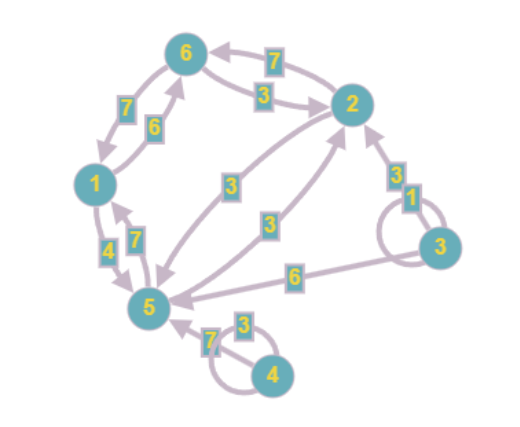
\includegraphics[width=0.5\linewidth]{4idz_1.png}
    \caption{}
    \label{fig:enter-label}
\end{figure}
Получаем:\\
$E_0 = $ {3, 4}\\
$E_1 = $ {1, 2, 5, 6}\\
\end{proof}

%%%%%%%%%%%%%% ЗАДАНИЕ №3 %%%%%%%%%%%%%%
%% Условие задания №3
\begin{problem}
Есть ли невозвратные состояния?
\end{problem}

%% Решение задания №3
\begin{proof}
Да, есть, вершины: 3, 4\\
\end{proof}

%%%%%%%%%%%%%% ЗАДАНИЕ №4 %%%%%%%%%%%%%%
%% Условие задания №4
\begin{problem}
Найти период в каждом из классов.
\end{problem}

%% Решение задания №4
\begin{proof}
Матрица класса 1:
\[
P_1 = \frac{1}{10}\begin{pmatrix}
    0 & 0 & 4 & 6  \\
    0 & 0 & 3 & 7  \\
    7 & 3 & 0 & 0  \\
    7 & 3 & 0 & 0 \\
\end{pmatrix}
\]

\[
P_1^2 = \frac{1}{100}\begin{pmatrix}
    70 & 30 & 0 & 0  \\
    70 & 30 & 0 & 0  \\
    0 & 0 & 37 & 63  \\
    0 & 0 & 37 & 63 \\
\end{pmatrix}
\]
$\Rightarrow T = \text{НОД}(2) = 2\\$

\end{proof}

%%%%%%%%%%%%%% ЗАДАНИЕ №5 %%%%%%%%%%%%%%
%% Условие задания №5
\begin{problem}
Вычислить финальные вероятности в каждом классе.
\end{problem}

%% Решение задания №5
\begin{proof}
$E_1$:
\begin{gather*}
    x = (p_1, p_2, p_5, p_6)\\
    \begin{cases}
        (10P_1^T - 10I)x^T = 0 \\
        p_1 + p_2 + p_5 + p_6 = 1
    \end{cases} \Leftrightarrow \\
\end{gather*}

\[
\begin{pmatrix}
    -10 & 0 & 7 & 7 \\
    0 & -10 & 3 & 3 \\
    4 & 3 & -10 & 0 \\
    6 & 7 & 0 & -10 \\
\end{pmatrix}
\begin{pmatrix}
    p_1 \\
    p_2 \\
    p_5 \\
    p_6 \\
\end{pmatrix}
\Rightarrow
\]\\
$p_1 = \frac{7}{20}; p_2 = \frac{3}{20}; p_5 = \frac{37}{200}; p_6 = \frac{63}{200};\\$\\
$E_0:\\$
$p_3 = 0; p_4 = 0$.
\end{proof}
